% !TEX root = ../thesis.tex

\chapter{Case Study II: Medical Ultrasound Diagnosis} \label{chp:medical}

This chapter proposes a comprehensive validation of the CORTEX architecture in the medical domain, focusing on ultrasound diagnosis as a representative case of non-spatial Digital Twin applications. The case study demonstrates how the CORTEX framework can be adapted beyond geometric representations to support sophisticated reasoning about complex physiological systems.

\section{Clinical Decision-Making Challenges}

Medical ultrasound serves as one of the most widely used imaging modalities in modern healthcare across cardiology, obstetrics, emergency medicine, and other specialties. However, ultrasound diagnosis presents unique challenges: image quality highly depends on operator technique, real-time interpretation requires immediate decision-making, image interpretation requires extensive training experience, and significant inter-observer variability exists.

Current AI-assisted medical imaging systems typically operate as isolated tools providing specific diagnostic suggestions without integration into broader clinical reasoning processes. The CORTEX approach addresses this limitation by providing a comprehensive clinical reasoning framework that integrates image analysis with broader medical knowledge and reasoning capabilities.

\section{Non-Visual Digital Twin Design}

The medical ultrasound case demonstrates a fundamentally different approach to Digital Twin representation compared to geometric models used in building monitoring or UAV exploration. This approach operates in high-dimensional feature spaces that capture essential diagnostic information from ultrasound images while enabling sophisticated reasoning about medical conditions and treatment options.

\begin{figure}[htbp]
\centering
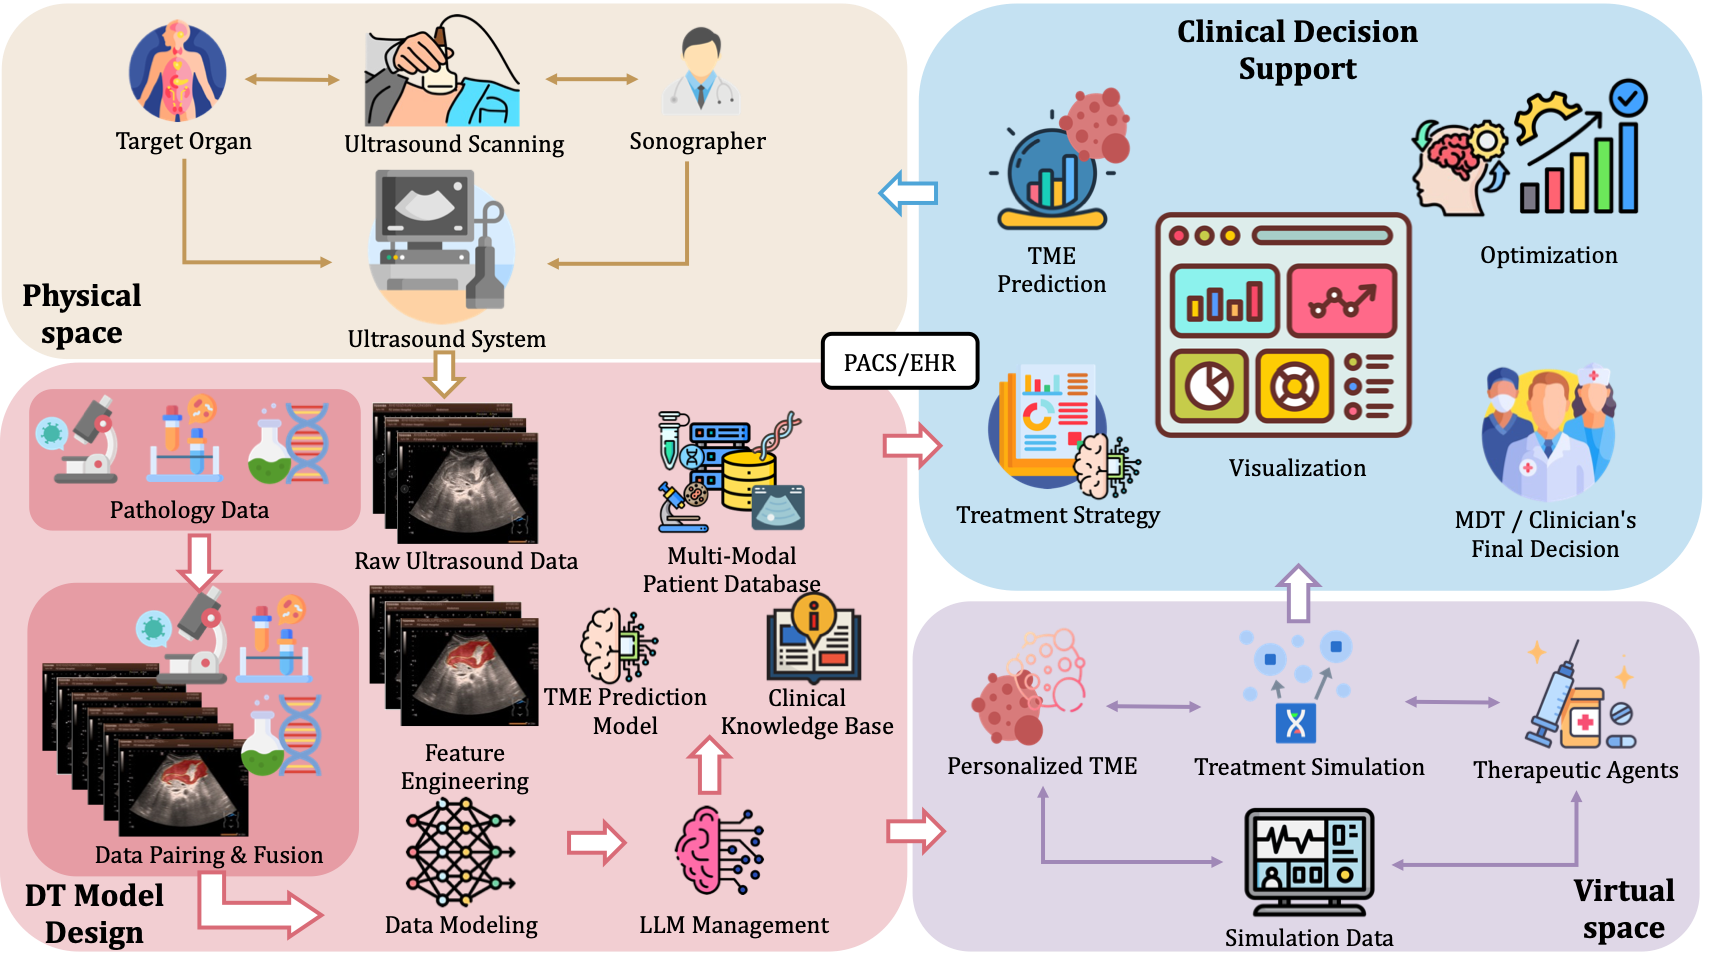
\includegraphics[width=0.8\textwidth]{figures/Med/med_framework.png}
\caption{Digital Twin architecture framework for medical ultrasound diagnosis. The framework shows the complete workflow from ultrasound scanning in physical space to clinical decision support in virtual space, including data pairing and fusion, Digital Twin model design, feature engineering, TME prediction model, and LLM management components.}
\label{fig:med_framework}
\end{figure}

\subsection{2D Ultrasound Feature Extraction}

\textbf{Completed Work}: Established deep learning feature extraction pipelines utilizing convolutional neural network architectures specifically adapted for medical ultrasound characteristics. Preprocessing stages normalize image intensity, reduce speckle noise, and enhance relevant anatomical structures. Multi-scale analysis captures fine-grained textural details relevant for specific pathological conditions and broader structural patterns characterizing normal and abnormal anatomy.

\textbf{Planned Implementation}:
\textbf{Domain-Specific Modifications}: Integrate attention mechanisms focusing on clinically relevant regions, specialized loss functions ensuring learned features correlate with clinically meaningful differences.
\textbf{Robustness Enhancement}: Implement adaptive mechanisms maintaining consistent performance across different image quality levels, develop artifact detection and mitigation algorithms.
\textbf{Uncertainty Modeling}: Explicitly represent uncertainty and confidence measures for each feature component.

\subsection{Multi-Dimensional Feature Space}

\textbf{Design Approach}: Extracted features will be organized into high-dimensional Digital Twin representations serving as cognitive interfaces between raw ultrasound data and clinical reasoning processes. Feature space construction integrates multiple types of extracted features into coherent, queryable structures organized according to clinical significance, temporal characteristics, and spatial relationships within ultrasound images.

\textbf{Key Technical Requirements}:
\textbf{Semantic Organization}: Create meaningful groupings according to anatomical regions, physiological systems, and pathological processes.
\textbf{Temporal Evolution}: Track patient condition changes over time, identify disease progression or treatment response patterns.
\textbf{Clinical Metadata Integration}: Integrate patient demographic information, clinical history, current symptoms, laboratory results.

\section{CORTEX Medical Adaptation}

The adaptation of CORTEX architecture for medical ultrasound diagnosis requires specialized modifications addressing unique clinical decision-making requirements while maintaining core LLM-Digital Twin integration principles established in Chapter 3.

\subsection{Medical Four-Stage Loop}

\textbf{Stage 1: Clinical Assessment}: Automated extraction and analysis of relevant clinical information from multiple sources including current ultrasound images, patient medical history, presenting symptoms, laboratory results, and previous imaging studies.

\textbf{Stage 2: Differential Diagnosis}: Generate comprehensive differential diagnosis lists based on observed clinical features and imaging findings, ranking potential diagnoses according to likelihood and clinical significance.

\textbf{Stage 3: Diagnostic Recommendations}: Generate specific diagnostic recommendations with detailed confidence estimates and supporting evidence. Recommendations include primary diagnostic conclusions and suggestions for additional testing, follow-up procedures, or specialist consultation when appropriate.

\textbf{Stage 4: Clinical Feedback Integration}: Collect and process feedback from multiple sources including immediate validation of diagnostic recommendations by clinical experts, longer-term patient outcome tracking, and systematic analysis of diagnostic accuracy across different case types.

\begin{figure}[htbp]
\centering
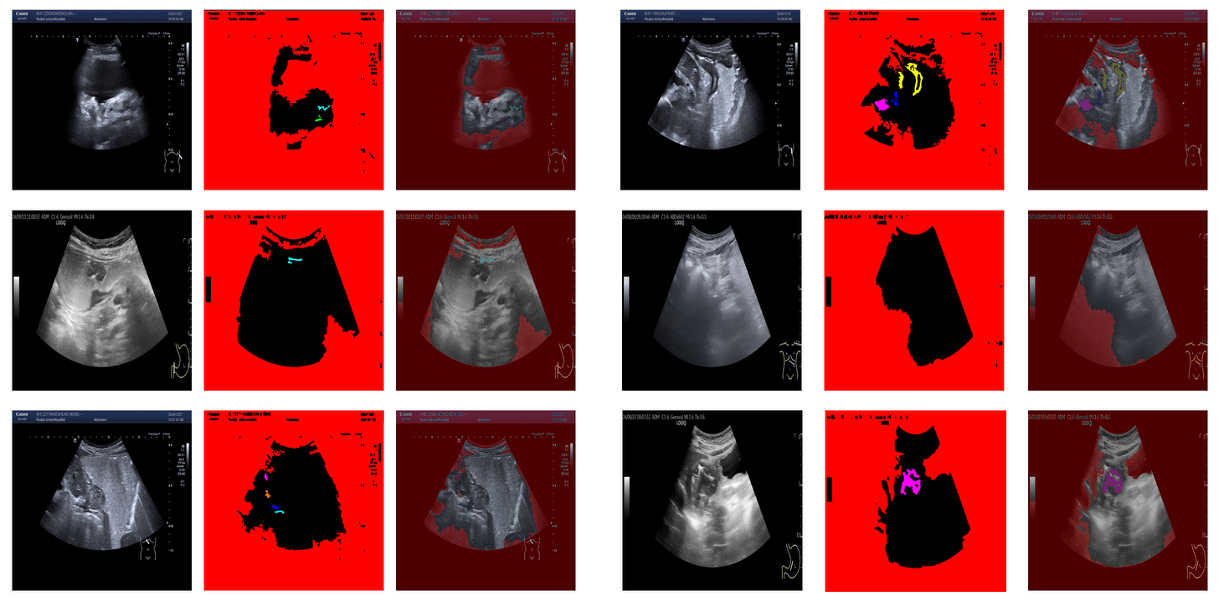
\includegraphics[width=0.9\textwidth]{figures/Med/medsam_result.png}
\caption{Medical image segmentation and analysis results. The images show original images, segmentation results, and overlay displays for different types of medical ultrasound images, demonstrating the system's identification and analysis capabilities across different anatomical structures and pathological conditions.}
\label{fig:medsam_result}
\end{figure}

\subsection{Clinical Reasoning Integration}

\textbf{Medical Language Model Fine-tuning}: Utilize high-quality medical text corpora including medical textbooks, clinical guidelines, peer-reviewed literature, and anonymized clinical case studies for specialized training processes. Evaluation protocols specifically designed for medical AI applications assess model performance on clinical reasoning tasks, medical knowledge comprehension, and ability to generate clinically appropriate recommendations.

\textbf{Clinical Reasoning Generation}: Leverage adapted LLM enhanced medical knowledge to support sophisticated clinical decision-making processes. System generates detailed reasoning traces following established clinical reasoning patterns, including systematic consideration of differential diagnoses, evaluation of supporting and contradicting evidence, and integration of multiple information sources.

\textbf{Planned Implementation}:
\textbf{Natural Language Interaction}: Develop intuitive interfaces supporting effective communication between healthcare professionals and AI systems.
\textbf{EHR Integration}: Achieve seamless integration with electronic health records, addressing data interoperability, security requirements, and clinical workflow integration challenges.
\textbf{Real-time Reasoning}: Optimize reasoning speed to meet clinical environment time requirements.

\section{Safety and Ethics}

\textbf{Patient Privacy Protection}: Implement HIPAA compliance requirements through comprehensive technical and procedural safeguards. Advanced encryption and access control mechanisms protect patient data, while de-identification and anonymization procedures ensure patient privacy protection in research activities.

\textbf{Clinical Safety Protocols}: Provide multiple layers of protection against potential AI system failures or inappropriate recommendations. Safety framework includes explicit bounds checking identifying potentially dangerous recommendations, ensuring critical clinical decisions maintain appropriate human supervision.

\textbf{Bias Detection and Fairness}: Address critical concerns that AI systems may perpetuate or amplify existing healthcare disparities. Bias detection framework includes systematic monitoring of system performance across different demographic groups to identify potential fairness concerns.

\section{Experimental Design}

\subsection{Clinical Collaboration}

\textbf{Multi-center Data Collection}: Plan collaboration with multiple healthcare institutions including academic medical centers, community hospitals, and specialty clinics to capture the full spectrum of clinical presentations and practice patterns.

\textbf{Ground Truth Establishment}: Provide essential reference standards for rigorous AI system evaluation through expert consensus. Consensus process involves multiple expert radiologists and clinicians independently reviewing each case.

\textbf{Implementation Plan}:
\textbf{Phase 1} (Completed): Complete ethical review and data collection protocol development.
\textbf{Phase 2} (Ongoing): Feature extraction algorithm development and preliminary validation.
\textbf{Phase 3} (Planned): Large-scale clinical data collection and annotation.
\textbf{Phase 4} (Planned): System integration testing and clinical pilot studies.

\subsection{Evaluation Framework}

\textbf{Diagnostic Accuracy Assessment}: Employ multiple accuracy metrics assessing system ability to correctly identify pathological conditions and distinguish normal presentations, including overall accuracy, class-specific accuracy, and performance analysis across different diagnostic certainty levels.

\textbf{Clinical Utility Assessment}: Evaluate practical value of AI-assisted diagnosis in real clinical settings, including healthcare professional diagnostic confidence improvement, diagnostic workflow time savings, and reduction in diagnostic errors and missed cases.

\textbf{Expected Results}:
\textbf{Accuracy Improvement}: 12-18% diagnostic accuracy improvement compared to traditional CAD systems.
\textbf{Efficiency Enhancement}: 15-25% overall time savings for routine diagnostic cases.
\textbf{Consistency Enhancement}: Improved expert clinical assessment consistency (kappa > 0.75).

\section{Clinical Implications}

\subsection{Clinical Value Assessment}

The potential clinical value of the CORTEX medical diagnostic system encompasses multiple healthcare improvement dimensions:

\textbf{Diagnostic Consistency Improvement}: Address substantial inter-observer variability characterizing medical imaging interpretations. Systematic diagnostic reasoning approach helps standardize diagnostic approaches across different practitioners and clinical settings.

\textbf{Support for Less Experienced Practitioners}: Provide valuable support for practitioners who may lack extensive experience for confident interpretation of challenging cases. Comprehensive reasoning capabilities and uncertainty quantification provide immediate decision support for complex diagnostic scenarios.

\textbf{Healthcare Cost-Effectiveness}: Achieve significant cost savings and improved resource utilization through improved diagnostic efficiency, reduced unnecessary follow-up testing, and optimized specialist consultation patterns.

\subsection{Technical Challenges}

\textbf{Key Technical Challenges}:
\textbf{Cross-Device Generalization}: Equipment differences and acquisition protocol variations across different ultrasound systems.
\textbf{Rare Pathology Handling}: Limited training data for rare disease diagnostic capabilities.
\textbf{Clinical IT Integration}: Complex integration requirements with diverse healthcare IT environments.
\textbf{Regulatory Compliance}: Strict regulatory framework compliance for medical AI systems.

\textbf{Future Research Directions}:
\textbf{Multi-modal Extension}: Extend to other medical imaging modalities such as CT, MRI, X-ray.
\textbf{Multi-modal Data Integration}: Integrate diverse clinical information including laboratory results, clinical notes, patient history.
\textbf{Personalized Medicine}: Adaptive diagnostic approaches based on patient-specific factors.
\textbf{Longitudinal Monitoring}: Temporal modeling capabilities supporting long-term patient care.

\section{Chapter Summary}

The medical ultrasound diagnosis case study successfully demonstrates the adaptability and effectiveness of the CORTEX cognitive architecture in safety-critical healthcare applications, providing important validation for the LLM-Digital Twin integration approach. The case study validates several key aspects of the CORTEX architecture: feasibility of non-visual Digital Twin representations based on high-dimensional feature spaces, effectiveness of domain-specific adaptation of the four-stage cognitive loop for clinical reasoning, and potential for significant improvements in diagnostic accuracy and clinical utility through systematic LLM-Digital Twin integration.

The clinical implications and translational potential extend beyond immediate diagnostic assistance to broader considerations of healthcare delivery, medical education, and the evolving role of AI in clinical practice. The system's potential to improve diagnostic consistency, support less experienced practitioners, and reduce diagnostic errors could have significant public health impact.

CORTEX's successful adaptation to medical diagnosis provides important preparation for the final case study examining autonomous UAV exploration, which will demonstrate the architecture's capabilities in dynamic, real-time physical world interaction. The progression from building health monitoring through medical diagnosis to autonomous exploration provides comprehensive validation of the CORTEX approach across diverse application domains.